\documentclass[12pt]{article}
\usepackage{amssymb,amsfonts,amsmath,graphicx,mathtools}
\usepackage[alphabetic,y2k,lite]{amsrefs}
\usepackage{fullpage, mystyle}
\usepackage{MnSymbol}

\usepackage{tikz}
\usepackage{tikz-cd}

\newcommand{\disk}[1]{{D^{#1}}}
\newcommand{\sphr}[1]{{S^{#1}}}
\newcommand{\empt}[1]{{\emptyset^{#1}}}

\newcommand{\VV}{{\mathbf{V}}}
\DeclareMathOperator{\Skein}{Skein}
\newcommand{\op}{{\text{op}}}
\newcommand{\wdtld}[1]{{\widetilde{#1}}}

\newcommand{\cB}{{\mathcal{B}}}
\newcommand{\hatbox}{{\hat{\boxtimes}}}

\DeclareMathOperator{\Set}{Set}
\DeclareMathOperator{\Vect}{Vec}

\begin{document}

\title{Upgrading an $(n+\veps)$-TQFT to an extended $(n+1)$-TQFT}
\author{Ying Hong Tham}
\date{25 December, 2022}
\maketitle


In this note, we show that one can promote an
$(n+\veps)$-TQFT to an extended $(n+1)$-TQFT
by only specifying the value associated to
the $(n+1)$-disk $Z(\disk{n+1}) \in Z(S^n)$.

Suppose we are given an $(n+\veps)$-TQFT $Z$,
that is,
it assigns a category $Z(N)$ to a closed $(n-1)$-manifold $N$,
and a functor $Z(M):Z(N) \to Z(N')$ to an $n$-dimensional
cobordisms $M:N\to N'$ between $(n-1)$-manifolds.

TODO perhaps comment on requirements on $Z$,
e.g. a natural isom for $M \simeq M'$,
especially for $Z(M' \circ M) \simeq Z(M') \circ Z(M)$
that is consistent.
Or say, at this point, no assumption on existence of
adjointness of functors $Z(M) \dashv Z(\ov{M})$.

The empty $k$-manifold is denoted by $\empt{k}$.
Composition of cobordisms is written from right to left,
so composition of $M: N \to N'$ and $M' : N' \to N''$
is denoted by $M' \circ M: N \to N''$.

2-Cob denotes the bicategory with
closed $(n-1)$-manifolds as objects,
$n$-dimensional cobordisms as 1-morphisms,
and $(n+1)$-dimensional relative cobordisms as 2-morphisms.

\begin{proposition}
\label{p:extend-uniqueness}
Consider functors
$Z(\disk{n}) : Z(\empt{n-1}) \rightleftharpoons
	Z(\sphr{n-1}) : Z(\ov{\disk{n}})$.

Let $\eta_0: Z(\empt{n}) \Rightarrow
	Z(\sphr{n} = \ov{\disk{n}} \circ \disk{n})
	: Z(\empt{n-1}) \to Z(\empt{n-1})$
be a natural transformation,
and suppose it is the unit to an adjunction
$Z(\disk{n}) \dashv Z(\ov{\disk{n}})$.

Then if $Z',Z''$ are extended $(n+1)$-TQFTs
such that $Z',Z''$ agree with $Z$ on $(n-1)$- and $n$-manifolds,
and $Z'(\disk{n+1}) = Z''(\disk{n+1}) = \eta_0$,
then $Z' \cong Z''$.
\end{proposition}


\begin{proof}
From the topology section below,
we know that a 2-morphism of 2-Cob that realizes
the attachment of an $(n+1)$-dim $(k+1)$-handle,$0 \leq k \leq n$,
is determined by some counit $\veps_k$
of an adjunction,
whose corresponding unit can be built from handles
of index at most $k$,
and thus, the value of extensions $Z'$ of $Z$ on 2-morphisms
is completely determined by its value on the
$(n+1)$-dim 0-handle, which is exactly $\eta_0$.
\end{proof}



\section{Topology}

\subsection{Adjunctions from topology}
\label{s:topology-adjunctions}

For the purposes of the proof of the proposition above,
only the first simple example from this section is needed,
the reader may then skip to \secref{s:handles-from-adjunctions}.

In 2-Cob,
%In the 2-category with closed $(n-1)$-manifolds as objects,
%$n$-dimensional cobordisms as 1-morphisms,
%and $(n+1)$-dimensional relative cobordisms as 2-morphisms,
the $n$-dimensional cobordisms
$M: N \rightleftharpoons N' : \ov{M}$
form an adjunction.

Let us first consider a simple case,
which is the main setting in \prpref{p:extend-uniqueness}.
Consider $n$-dim cobordisms
$\disk{n}: \empt{n-1} \rightleftharpoons
	\sphr{n-1}: \ov{\disk{n}}$.
This can be promoted to an adjunction
$\disk{n} \dashv \ov{\disk{n}}$
with the following unit and counit 2-morphisms:
the unit is given by the $(n+1)$-disk
$\disk{n+1}: \empt{n} \Rightarrow
	(\ov{\disk{n}} \circ \disk{n}) = \sphr{n}$,
and the counit is given by the $(n+1)$-disk which,
as a manifold with corner $\sphr{0} \times \sphr{n-1}$,
is a 2-morphism
$\disk{n+1} = I \times \disk{n}: \disk{n} \circ \ov{\disk{n}}
	\Rightarrow I \times \sphr{n-1} = \id_{\sphr{n-1}}$.
This is easily checked to be an adjunction,
the unit is an $(n+1)$-dimensional 0-handle,
and the counit is attaching an $(n+1)$-dimensional 1-handle
to $\disk{n} \sqcup \ov{\disk{n}}$
(see \figref{f:disk-adjunction} for $n=1$ case).

\begin{figure}[ht]
\rotatebox[origin=c]{180}{
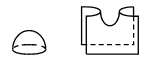
\includegraphics[width=6cm]{disk-adjunction-unit-counit.png}
}
\hspace{20pt};
\hspace{20pt}
\rotatebox[origin=c]{180}{
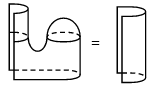
\includegraphics[width=6cm]{disk-adjunction-snake-equation.png}
}
\caption{Counit and unit for adjunction
$\disk{n}: \empt{n-1} \rightleftharpoons
	\sphr{n-1}: \ov{\disk{n}}$,
for $n=1$,
along with one of the snake equations;
relative cobordism goes up
(stolen from \cite{SPries},
Figure 1.6 and 1.10, get rotated)}
\label{f:disk-adjunction}
\end{figure}


Now consider $M: N \rightleftharpoons N': \ov{M}$,
where $M$ is an elementary cobordism of index $k$,
i.e. it is obtained from $N \times I$
by attaching a $k$-handle.
Then $\ov{M}$ is the dual elementary cobordism
which is of index $n-k$.
[See \figref{f:dual-handle}]

\begin{figure}[ht]
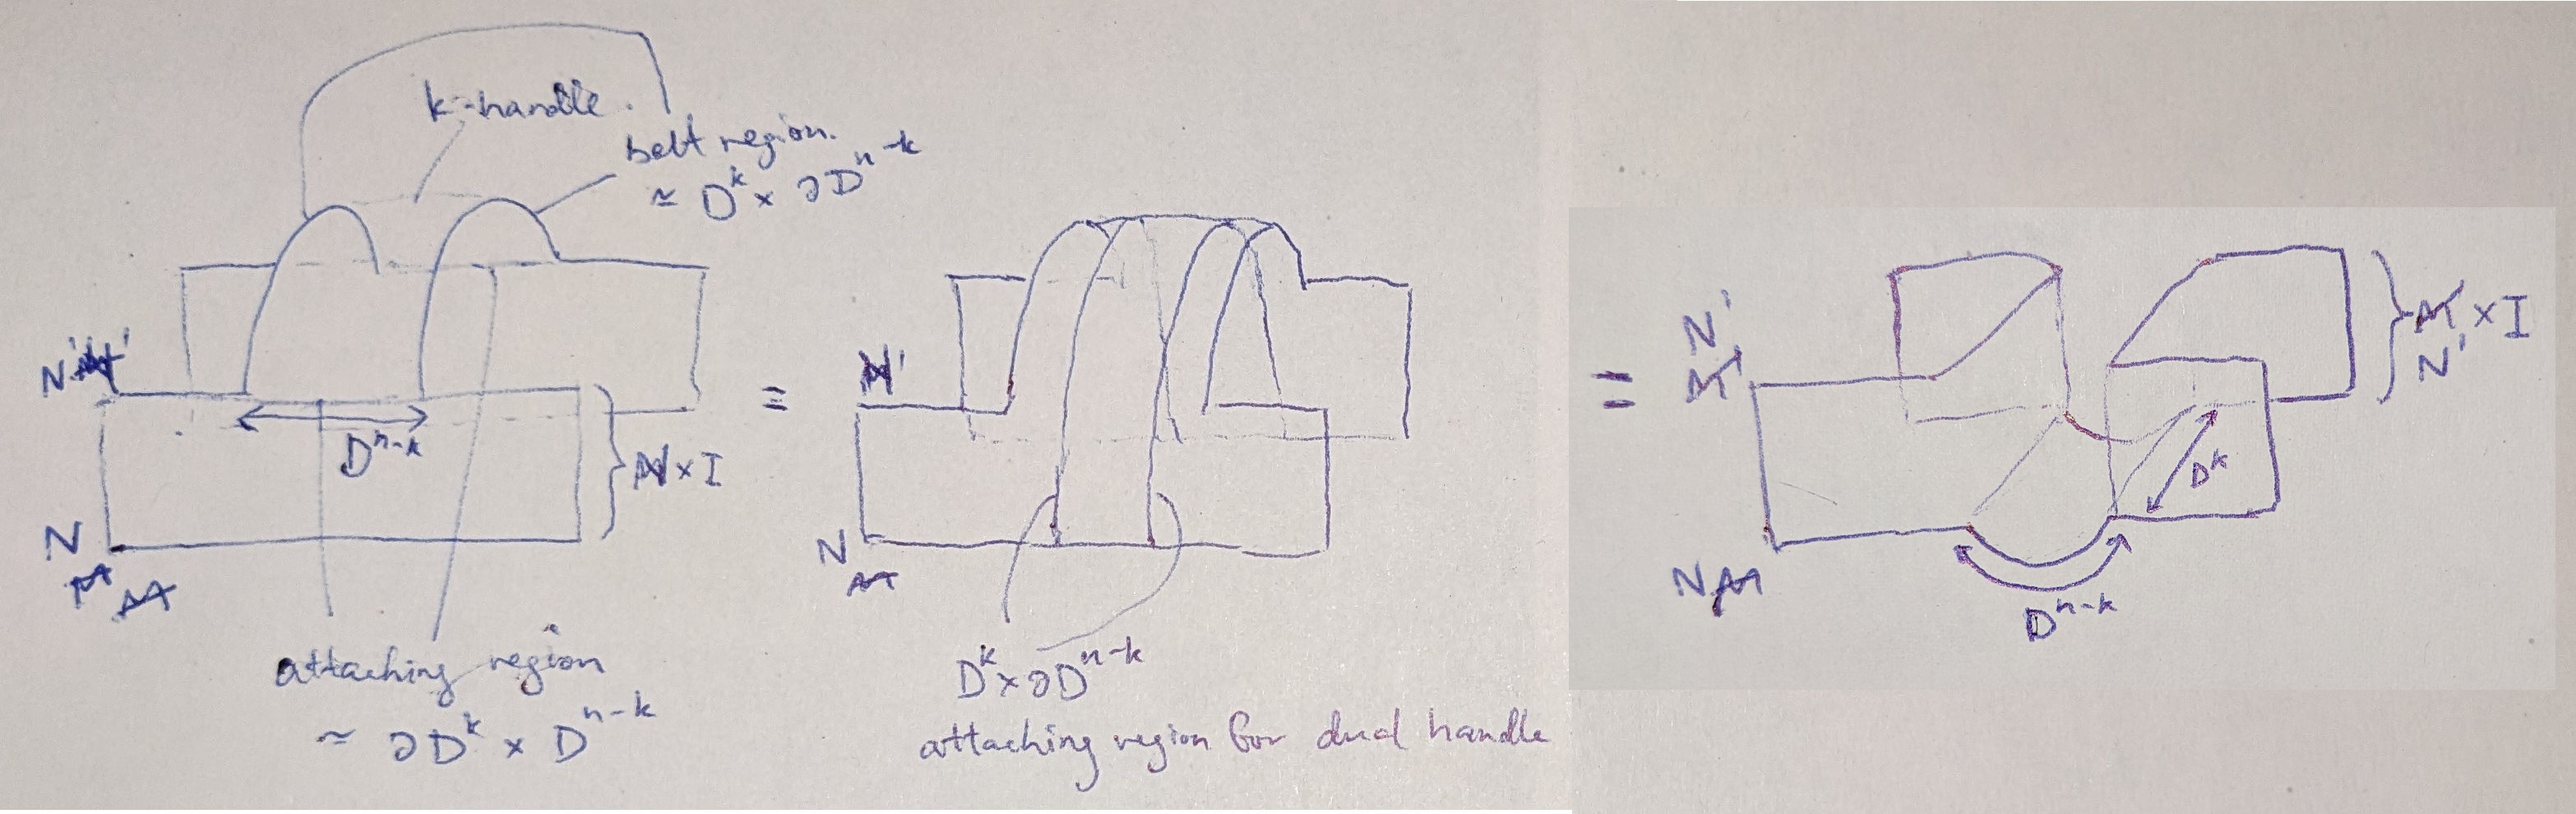
\includegraphics[width=15cm]{diagram-dual-handle.jpg}
\caption{$M:N \to N'$ is an elementary cobordism
of index $k$; it is built from attaching a disk $\disk{n}$
to $N \times I$,
with attaching region $\del \disk{k} \times \disk{n-k}$.
It can also be built from the other direction,
by attaching a disk $\disk{n}$
to $N' \times I$,
with attaching region $\disk{k} \times \del \disk{n-k}$.
Thus, turning it upside-down, i.e.
treated as a cobordism $\ov{M}: N' \to N$,
it is an elementary cobordism of index $(n-k)$.
}
\label{f:dual-handle}
\end{figure}

[See \figref{f:elementary-cobord-counit-unit}]
We construct the counit
$\veps: M \circ \ov{M} \Rightarrow \id_{N'} : N' \to N'$
by attaching an
$(n+1)$-dimensional $(k+1)$-handle to $M \cup_{N'} \ov{M}$,
with attaching region being essentially the
$k$-handle in $M$ plus the $(n-k)$-handle in $\ov{M}$;
the attaching sphere is the union of the core of the
$k$-handle in $M$
with the co-core of the $(n-k)$-handle in $\ov{M}$.
Similarly,
we construct the unit
$\eta: \id_N \Rightarrow M \circ \ov{M} : N \to N$
by attaching an
$(n+1)$-dimensional $k$-handle to $\id_N = N \times I$;
the attaching region for this $(n+1)$-dim $k$-handle
is
$($the attaching region for the $n$-dim $k$-handle that defines
$M) \times I$.
The snake equations
$\id_M = (\veps \circ M) \cdot (M \circ \eta):
M \Rightarrow M \circ \ov{M} \circ M \Rightarrow M$
and
$\id_{\ov{M}} = (\ov{M} \circ \eta) \cdot (\eta \circ \ov{M}):
\ov{M} \Rightarrow \ov{M} \circ M \circ \ov{M} \Rightarrow \ov{M}$
follow from the fact that
these $(n+1)$-dim handles form a cancelling pair
in both cases.

Here we have $M \dashv \ov{M}$,
but we may very well have $\ov{M} \dashv M$;
the counit $\veps': \ov{M} \circ M \Rightarrow \id_N$
is an $(n+1)$-dim elementary cobordism
of index $(n-k+1)$.
It is interesting to note that
this counit is the dual cobordism to the unit
$\eta: \id_N \Rightarrow \ov{M} \circ M$
previously described.

\begin{figure}[ht]
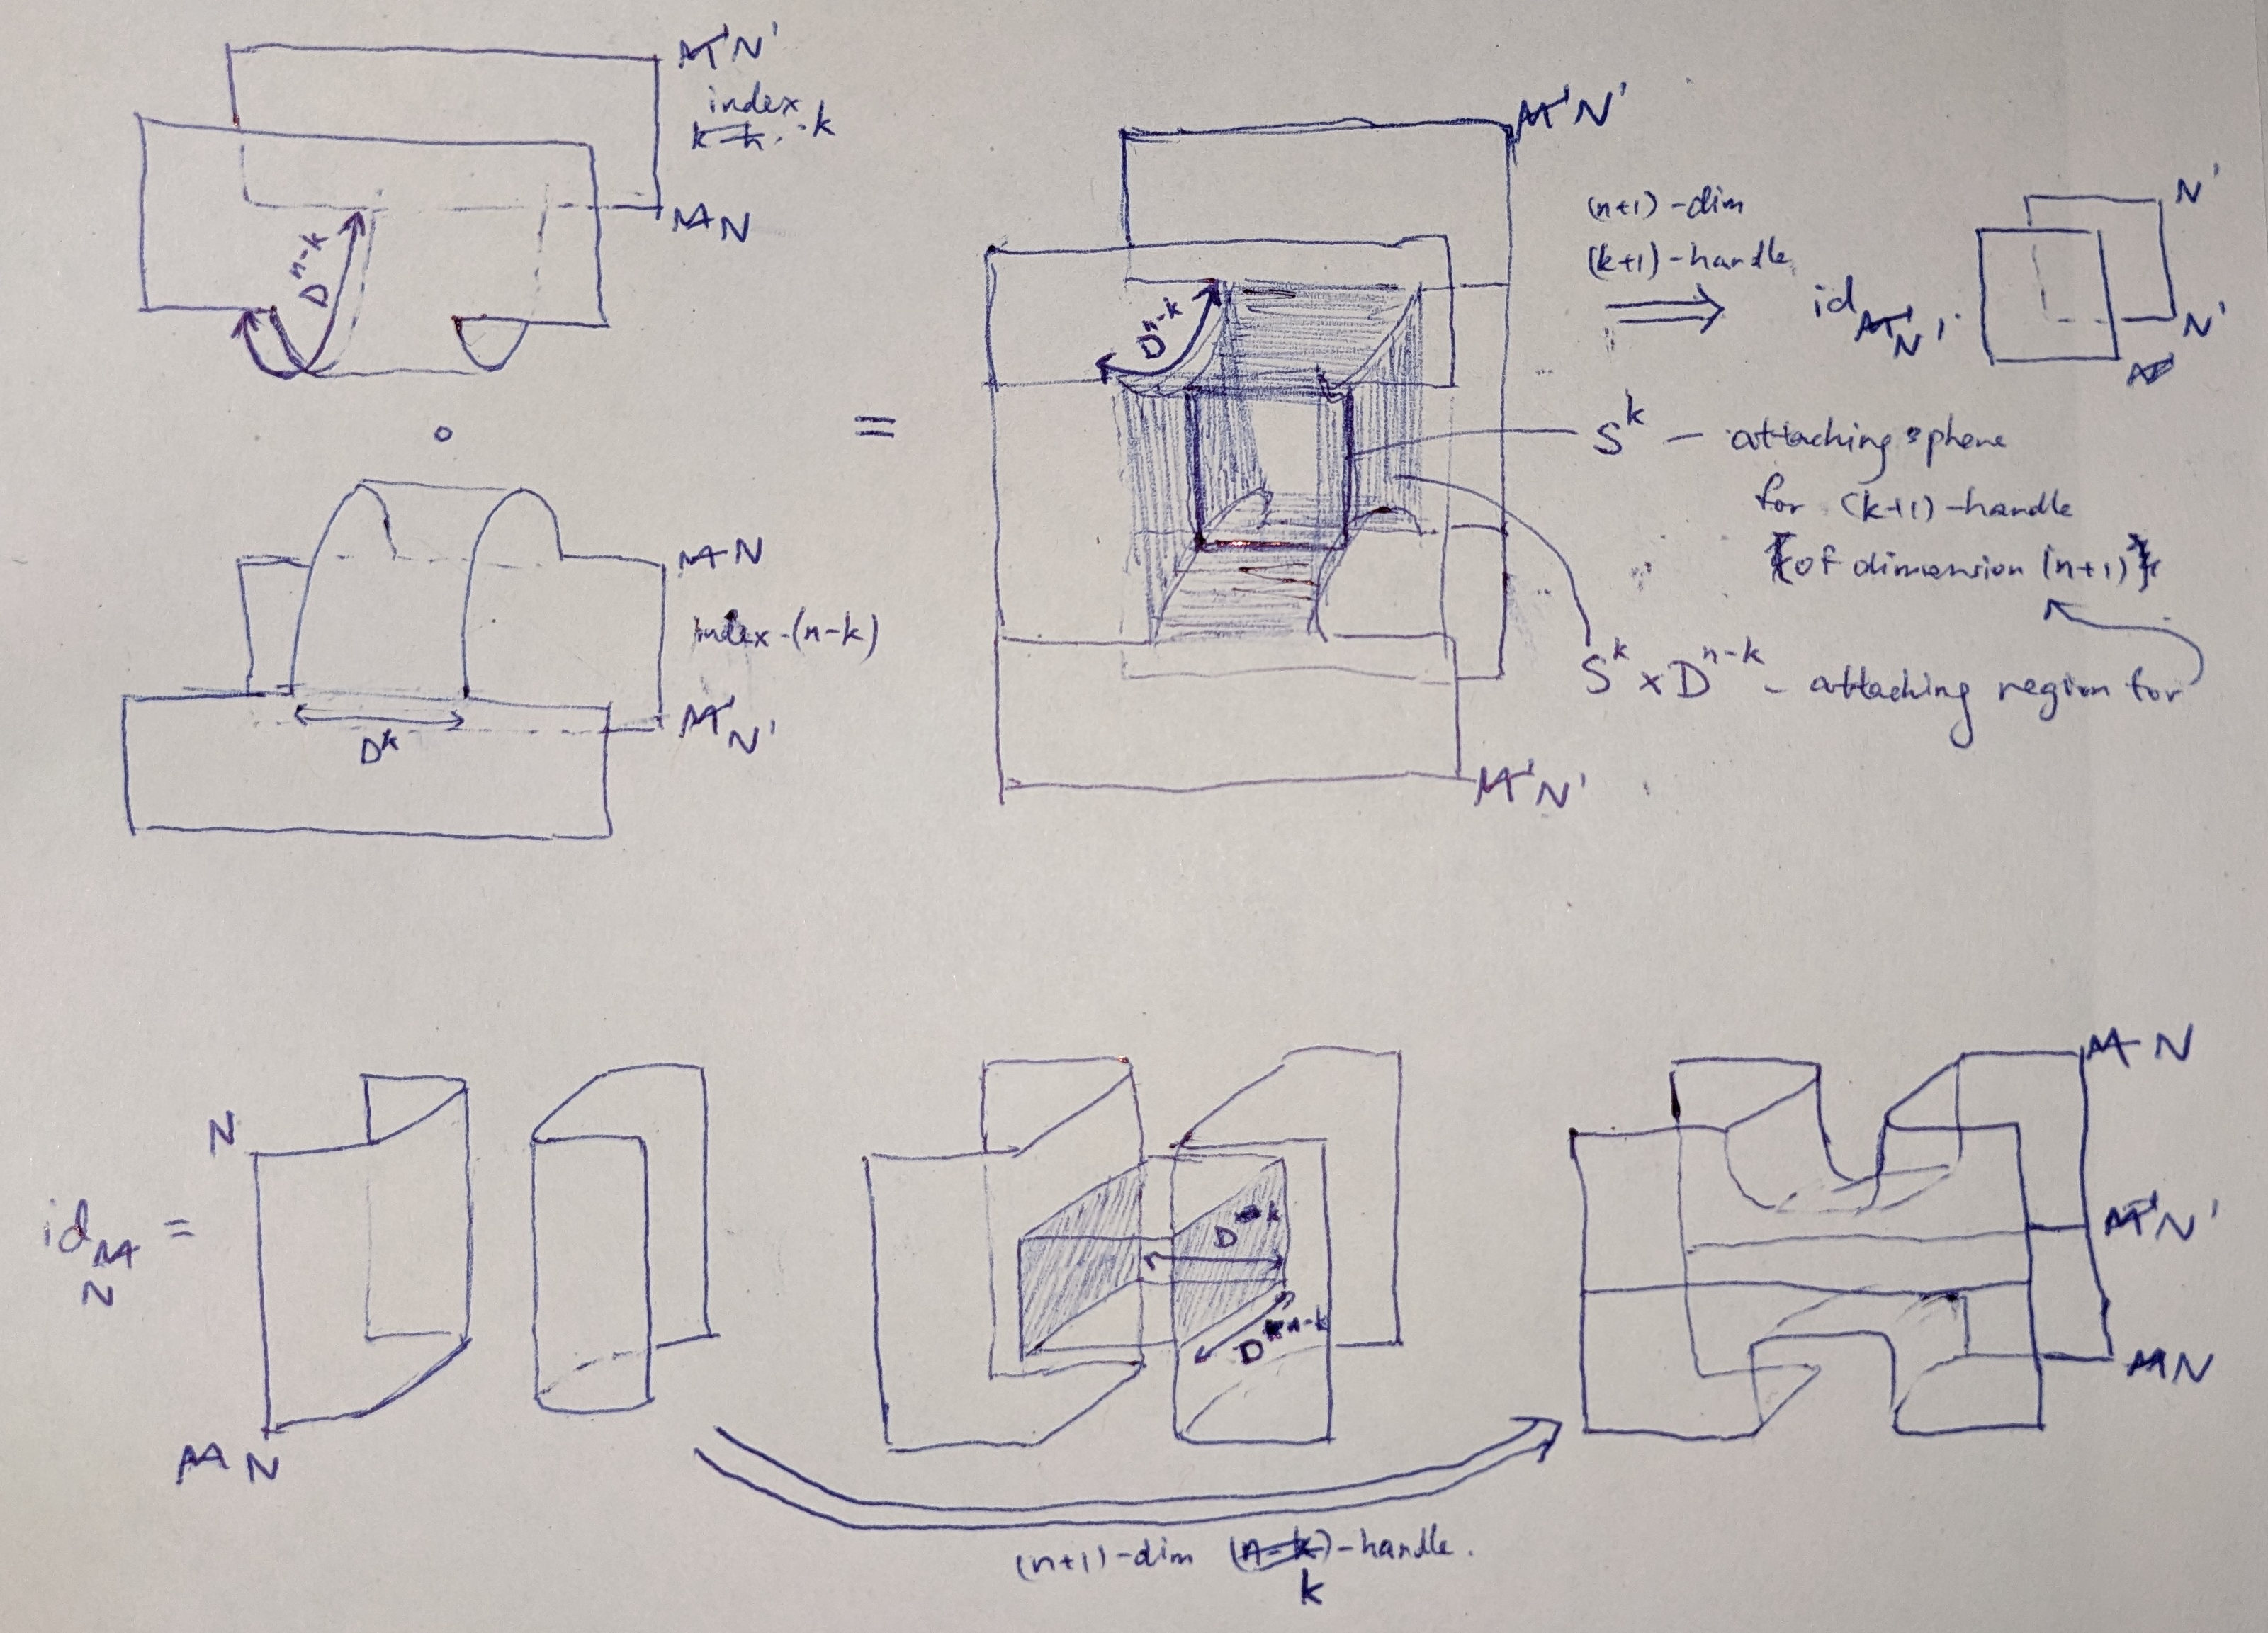
\includegraphics[width=15cm]{diagram-counit-unit-elementary-cobord.jpg}
\caption{Counit (top) and unit (bottom) for adjunction
$M: N \rightleftharpoons N': \ov{M}$,
where $M$ is an elementary cobordism of index $k$.
Note the way $N$ is drawn here looks like $N'$
in \figref{f:dual-handle} and vice versa
(by accident, sorry for minor confusion)}
\label{f:elementary-cobord-counit-unit}
\end{figure}



In general, we may consider the pair of $n$-dim cobordisms
$M : N \rightleftharpoons N': \ov{M}$.
By presenting $M$ as a composition of elementary cobordisms,
we may compose the adjunctions constructed
for each of these elementary cobordisms as above,
and obtain an adjunction $M \dashv \ov{M}$.



\begin{remark}
In \cite{Yprod},
we considered this construction
without realizing their connection to these adjunctions;
there we consider the more general case where
$N,N'$ may have (possibly different) boundary, and
$M: N \to N'$ is a relative cobordism
(with the boundary cobordism that is
not necessarily the identity cobordism).
\end{remark}


\subsection{Producing $(n+1)$-dim $k$-handles
from some adjunctions}
\label{s:handles-from-adjunctions}

Throughout this section, $0 \leq k < n$.

We show how to construct the $(n+1)$-dim $(k+1)$-handle
from the counit $\veps_k$ of the adjunction
$\sphr{k} \times \disk{n-k} : \empt{n} \rightleftharpoons
	\sphr{k} \times \sphr{n-k-1} : \ov{\sphr{k} \times \disk{n-k}}$
and the unit $\eta_0$ of the adjunction
$\disk{n} : \empt{n-1} \rightleftharpoons
	\sphr{n-1}: \ov{\disk{n}}$.
(The 0-handle is already given by $\eta_0$,
while the $(n+1)$-handle is the counit to the adjunction
$\ov{\disk{n}} : \sphr{n-1} \rightleftharpoons
	\empt{n-1}: \disk{n}$;
we say a few more words about this at the end of this section.)


The process of attaching a $(k+1)$-handle to an $(n+1)$-manifold
can be implemented as postcomposing by a 2-morphism.
More precisely, given an $(n+1)$-manifold $W$
presented as a 2-morphism $W: M \Rightarrow M' : N \to N'$,
and an attaching region $\sphr{k} \times \disk{n-k}$ in $M'$,
the $(n+1)$-manifold $W'$ obtained from
attaching a $(k+1)$-handle along the specified attaching region
may be considered as a 2-morphism
$W': M \Rightarrow M'': N \to N'$,
where $M''$ is obtain from $M'$ by performing surgery
along the attaching region
(cutting it out and gluing in $\disk{k+1} \times \sphr{n-k-1}$);
then $W' = \omega_{k+1} \cdot W$,
where $\omega_{k+1}$ is a 2-morphism that we will describe below.


Our 2-morphism $\omega_{k+1}$ is of the form
$\omega_{k+1}: \sphr{k} \times \disk{n-k}
	\Rightarrow \disk{k+1} \times \sphr{n-k-1} :
	\sphr{k} \times \sphr{n-k-1} \to \empt{n-1}$.
Since this is unchanged as $W$ varies,
we clearly need to make some arrangements
in order to use $\omega_{k+1}$.
More specifically,
we need to present $M'$ as a composition
\[
(\id_{N'} \sqcup \ov{\sphr{k} \times \disk{n-k}})
\circ (M \backslash \ov{\sphr{k} \times \disk{n-k}}) :
N \to N' \sqcup \sphr{k} \times \sphr{n-k+1} \to N'
\]
which is always possible by basic Morse theory.
So we have
($M^\circ := M \backslash \ov{\sphr{k} \times \disk{n-k}}$):

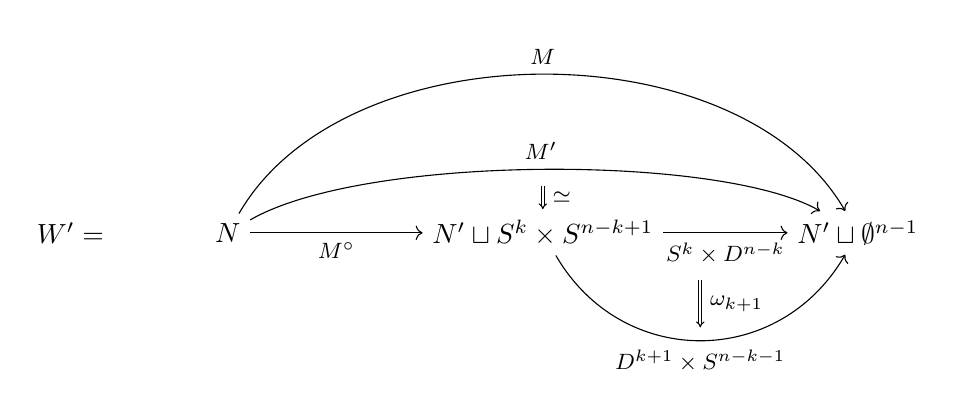
\begin{tikzpicture}
\node at (-2,0) {$W' = $};
% objects
\node (a) at (0,0) {$N$};
\node (b) at (4,0) {$N' \sqcup \sphr{k} \times \sphr{n-k+1}$};
\node (c) at (8,0) {$N' \sqcup \empt{n-1}$};
% 1-morph
\draw[->] (a) -- (b)
	node[pos=0.5,below] {\footnotesize $M^\circ$};
\draw[->] (b) -- (c)
	node[pos=0.5,below]
	{\footnotesize $\ov{\sphr{k} \times \disk{n-k}}$};
\draw[->] (b) .. controls +(-60:2cm) and +(-120:2cm) .. (c)
	node[pos=0.5,below]
	{\footnotesize $\ov{\disk{k+1} \times \sphr{n-k-1}}$};
\draw[->] (a) .. controls +(60:3cm) and +(120:3cm) .. (c)
	node[pos=0.5,above] {\footnotesize $M$};
\draw[->] (a) .. controls +(30:2cm) and +(150:2cm) .. (c)
	node[pos=0.5,above] {\footnotesize $M'$};
% 2-morph
\draw[-{Implies},double] (4,0.6) -- (4,0.3)
	node[pos=0.5,right] {\footnotesize $\simeq$};
\draw[-{Implies},double] (6,-0.6) -- (6,-1.2)
	node[pos=0.5,right] {\footnotesize $\omega_{k+1}$};
\end{tikzpicture}


Now let us describe how to construct $\omega_{k+1}$
out of $\veps_k$ and $\eta_0$,
which are, as a reminder,
the counit and unit of the adjunctions
$\sphr{k} \times \disk{n-k} : \empt{n} \rightleftharpoons
	\sphr{k} \times \sphr{n-k-1} : \ov{\sphr{k} \times \disk{n-k}}$
and
$\disk{n} : \empt{n-1} \rightleftharpoons
	\sphr{n-1}: \ov{\disk{n}}$,
respectively.

We may consider $\sphr{n}: \empt{n-1} \to \empt{n-1}$
as the composition $\ov{\disk{k+1} \times \sphr{n-k-1}}
\circ \sphr{k} \times \disk{n-k} :
\empt{n-1} \to \sphr{k} \times \sphr{n-k-1} \to \empt{n-1}$.

Then $\omega_{k+1}$ is given by the composition of 2-morphisms
\[
\omega_{k+1} = (\id_{\ov{\disk{k+1} \times \sphr{n-k-1}}}
		\circ \veps_k)
	\cdot (\id_{\ov{\sphr{k} \times \disk{n-k}}} \circ \eta_0)
\]

\begin{tikzpicture}
\node at (-2,0) {$\omega_{k+1} = $};
% objects
\node (a) at (0,0) {$\sphr{k} \times \sphr{n-k-1}$};
\node (b) at (4,0) {$\empt{n-1}$};
\node (c) at (8,0) {$\sphr{k} \times \sphr{n-k-1}$};
\node (d) at (12,0) {$\empt{n-1}$};
% 1-morph
\draw[->] (a) -- (b)
	node[pos=0.5,above] {\footnotesize $\ov{\sphr{k} \times \disk{n-k}}$};
\draw[->] (b) -- (c)
	node[pos=0.5,above] {\footnotesize $\sphr{k} \times \disk{n-k}$};
\draw[->] (c) -- (d)
	node[pos=0.5,above] {\footnotesize $\ov{\disk{k+1} \times \sphr{n-k-1}}$};
\draw[->] (b) .. controls +(60:3cm) and +(120:3cm) .. (d)
	node[pos=0.5,above] {\footnotesize $\empt{n}$};
\draw[->] (a) .. controls +(-60:3cm) and +(-120:3cm) .. (c)
	node[pos=0.5,above] {\footnotesize $\id_{\sphr{k} \times \sphr{n-k-1}}$};
% 2-morph
\draw[-{Implies},double] (8,1.6) -- (8,0.5)
	node[pos=0.5,right] {\footnotesize $\eta_0$};
\draw[-{Implies},double] (4,-0.5) -- (4,-1.4)
	node[pos=0.5,right] {\footnotesize $\veps_k$};
\end{tikzpicture}


A few words on the $(n+1)$-handle,
more generally the adjunction
$\ov{\disk{n}} : \sphr{n-1} \rightleftharpoons
	\empt{n-1}: \disk{n}$.
The unit is a 2-morphism
$\eta: \id_{\sphr{n-1}} \Rightarrow \disk{n} \circ \ov{\disk{n}}$,
which is clearly an elementary cobordism of index $n$.

A similar phenomenon happens with $\veps_k$,
that is, $\eta_k$, the unit to the adjunction
$\sphr{k} \times \disk{n-k} \dashv
	\ov{\sphr{k} \times \disk{n-k}}$,
to which $\veps_k$ is the counit,
is determined by handles of index at most $k$,
and indeed,
$\eta_k = \sphr{k} \times \disk{n-k+1}:
\empt{n} \Rightarrow \sphr{k} \times \sphr{n-k}:
\empt{n-1} \to \empt{n-1}$
is built from a 0-handle and a $k$-handle.


Thus, since the counit is uniquely determined by the unit,
the $(n+1)$-dim $k$-handle, for $k > 0$,
is determined by handles of lower index.
This may not be very useful in the topology world,
but on the algebraic side of a TQFT,
this means that everything is determined by the 0-handle.



[It may be helpful to note that the adjunction
$\sphr{k} \times \disk{n-k} : \empt{n} \rightleftharpoons
	\sphr{k} \times \sphr{n-k-1} : \ov{\sphr{k} \times \disk{n-k}}$
is simply $\sphr{k}$ times
the first example but with $n$ set to $n-k$,
$\disk{n-k} : \empt{n-k} \rightleftharpoons
	\sphr{n-1-k}: \ov{\disk{n-k}}$.
]


Note $\veps_k$ is not just a $k$-handle,
but may use lower $k$;
e.g. for $n = 3, k = 1$,
$\veps_k: \ov{S^1 \times D^2} \sqcup S^1 \times D^2 \Rightarrow
S^1 \times S^1 \times I$
uses one 1-handle (connecting the solid tori)
then a 2-handle.

%(Note that one can study the adjunction
%e.g. by considering the handle decomposition for
%$\sphr{k} \times \disk{n-k} : \empt{n} \to
%	\sphr{k} \times \sphr{n-k-1}$
%is given by a 0-handle followed by a $k$-handle,
%but this is 


\section{Profunctors}

Typically, to describe the $n$- and $(n-1)$- part of an
extended $(n+1)$-TQFT,
we need to assign a category $Z(N)$ to closed $(n-1)$-manifolds
and functors $Z(M): Z(N) \to Z(N')$
for an $n$-dimensional cobordism between $(n-1)$-manifolds
$N,N'$.

For skein theories (see \secref{s:skeins}),
it is more natural to describe the functor
associated to cobordisms in terms of a profunctor,
that is, in this case,
given any boundary value $\VV \in \Obj Z(N)$ at $N$
and $\VV' \in \Obj Z(N')$ at $N'$,
we assign some vector space $\wdtld{Z(M)}(\VV,\VV')$.
We may then convert this into a functor,
but this often requiring some additional choices.


In this section, we recall some basic results about
profunctors.

First, we will describe profunctors valued in $\Set$,
then profunctors valued in $\Vect$
for $\Vect$-enriched functors.

\begin{definition}
Let $\cA,\cB$ be categories.
A \emph{profunctor} $F$ from $\cA$ to $\cB$,
denoted $F: \cA \nto \cB$,
is a functor $F: \cB^\op \times \cA \to \Set$.
\end{definition}

\begin{example}
From a functor $G: \cA \to \cB$,
we may construct two profunctors
$G^*: \cA \nto \cB, G_*: \cB \nto \cA$,
defined by
\begin{align*}
G^* : \cB^\op \times \cA \to \Set
\hspace{30pt}
&;
\hspace{30pt}
G_* : \cA^\op \times \cB \to \Set
\\
(B, A) \mapsto \cB(B, GA)
\hspace{30pt}
&;
\hspace{30pt}
(A, B) \mapsto \cB(GA, B)
\end{align*}
\end{example}

\begin{definition}
Let $F: \cA \nto \cB, G: \cB \nto \cC$
be profunctors.
Their \emph{composition}
$G \circ F: \cA \nto \cC$
is given by
(assuming it exists, e.g. when $\cB$ is small):
\[
(G \circ F)(C,A) =
\int^B G(C,B) \times F(B,A)
=
\bigsqcup G(C,B) \times F(B,A) / \sim
\]
where the equivalence relation $\sim$
identifies $(y, F(b,\id_A)(x)) \sim (G(\id_C,b)(y),x)$
for $y \in G(C,B), x \in F(B,A), b: B \to B'$.
\end{definition}

One justification for defining composition as such is
the following (simple exercise on coends):
\begin{lemma}
The profunctor $\id_\cA^* = \cA(-,-)$ is
the identity for composition of profunctors,
i.e. for $F: \cA \nto \cB$,
$\id_\cB^* \circ F \simeq F \simeq F \circ \id_\cA^*$.
\end{lemma}

Perhaps a more philosophical reason for defining
composition of profunctors is from
their analogy with relations on sets.
In a sense, functors are to functions between sets
as profunctors are to relations between sets.
If $R \subseteq A \times B$ is a relation from $A$ to $B$
and $S \subseteq B \times C$ is a relation from $B$ to $C$,
their composition is
$S \circ R = \{(a,c) | \exists b: (a,b) \in R, (b,c) \in S\}$.


A more practical reason is that
this definition of composition is the standard (only?) trick
in category of ``doing everything''
when/if no extra choices are allowed to be made.

Yet another reason is the following.
Any object $B \in \cB$ defines a profunctor
$G \times_B F : \cA \nto \cC$,
by $(G \times_B F)(C,A) := G(C,B) \times F(B,A)$.
Any self-respecting composition $G \circ F$
should be a receptacle for this,
that is, refering back to the idea that profunctors are
analogs of relations,
if $G(C,B)$ and $F(B,A)$ are thought of as generalized arrows
from $B$ to $C$ and $B$ to $A$, respectively,
then we should be able to compose them,
so we should have a map
$G(C,B) \times F(B,A) \to (G\circ F)(C,A)$.
Moreover, if $B,B' \in \cC$ are related,
i.e. for morphism $b: B \to B'$,
$(G \times_B F)(C,A)$ and $(G \times_{B'} F)(C,A)$
should be related.
Hence coend.



=======
\subsection{In terms of generators and relations?}

Q: are there any more relations that need to be imposed
on the $(n+1)$-dim handles?


In \cite{SPries}, he presents $2,1,0$-Cob in terms of
generators and relations.
More specifically, there are four 1-morphisms,
tensoring them generates all 1-morphisms,
then there are two types of 2-morphism generators,
the invertible ones - cusps,
and the non-invertible ones - the 2-dim handles;
there are three types relations between 2-morphisms,
those involving only invertible 2-morphisms
- cusp relations and swallowtail,
those involving invertible and non-invertible - cusp flip,
and those involving the non-invertible 2-morphisms
- handle cancelations.

It seemed to me at first that the cusp flip relation could be
ignored if we define one type of 2d 1-handle
in terms of the other.
TODO picture.

However, it turns out this is not enough,
essentially because of symmetry.
In TODO figure, we see that we could have defined
the 1-handle using the last diagram instead of the second diagram;
but these are not equal unless we introduce the cusp flip relations.

An alternative is to define 1-handle in a way that,
I think, is more natural from a 2-dim perspective.
For the 0-manifold $N = (+,-,+,-)$,
there are two ways to realize a 1-morphism
$D^1 \times S^0 : N \to \emptyset$,
either pairing up the first two and last two points,
or pairing up the first and last and the middle two points
(by pair up I mean of course attaching $D^1$ to them);
a 2d 1-handle is a 2-morphism between them.

This approach is cleaner, and now the consequences
of the cusp flip relation
is taken care of by stipulating that this 2-morphism
is invariant under the $\ZZ/2$-symmetry of $N$
swapping $+$ and $+$, $-$ and $-$.

This symmetry would not exist if the objects (0-manifolds)
are ordered...

Upshot is that now we only need to types of relations of 2-morphisms,
those involving the invertible ones, and those involving only handles.

So this got me to wonder, can this be the case for higher dimensions?
If so, then this should prove that no additional relations are imposed
after the choice of $\eta_0$
(assuming all criteria on the $(n+\veps)$-theory needed to extended
are met; e.g. that some of these 1-morphisms are two-sided ``adjoint-able'').

I want to understand this in terms of generators and relations.

In extended $(n+1)$-Cob, there is sub-bicat,
same objects, 1-morphisms, but 2-morphisms are only invertible ones.

Suppose we understand this subcat in terms of generators and relations.
We can't hope to have a finite number of generators,
because in general there are infinitely many $(n-1)$-manifolds,
so we may consider finite number of ``types'' of generators or relations,
e.g. it is a $n$-dim $k$-handle.
That is, we have a finite collection of ``types'' of generating 1-morphisms,
a finite collection of ``types'' of generating 2-morphisms,
and we have a finite collection of ``types'' of relations among 2-morphisms,
such that for an $n$-manifold $M$,
presented as a composition of generating 1-morphisms in two ways, $f_1,f_2$,
and for $W = M \times I$,
presented as a composition of generating 2-morphisms in two ways,
$\vphi_1,\vphi_2: f_1 \Rightarrow f_2$,
there is a finite sequence of applications of the relations
that turns $\vphi_1$ into $\vphi_2$.





%%%%%%%%%%%%%%%%%%%%%%%%%%%%%%%%%%%%%%


========================================

%%%%%%%%%%%%%%%%%%%%%%%%%%%%%%%%%%%%%

Lawvere \cite{Lawvere} writes $\cA \bigotimes \cB$
for $\cA \hatbox \cB$ (he consideres profunctors enriched over
bicomplete symmetric monoidal closed category $\mathcal{V}$,
here we just take $\mathcal{V} = \Vect$).

Interesting example of profunctors

\begin{example}
A one-object $\Vect$-enriched category $*//A$
is simply an algebra.
Functors $F: *//A \to *//B$ are simply algebra homomorphisms,
and natural transformations are simply central elements of $B$.

On the other hand,
a profunctor $F: *//A \nto *//B$
is a functor $F: *//B^\op \times *//A \to \Vect$
(since $(*//B)^\op = *//B^\op$)
\end{example}


\section{Skein theory for $(1+\veps)$-theory}
\label{s:skeins}

To study completion of a $(n+\veps)$-theory
to an extended $(n+1)$-theory,
we start by studying the simplest case, $n = 1$.

In particular, we will study the $(1+\veps)$-theory
arising from skeins in 1-manifolds.

Manifolds with be assumed to be compact
unless otherwise specified.

We consider oriented 0-manifolds,
denoted by tuples of signs, e.g. $(+,+,-,+)$;
the empty 0-manifold is denoted by $()$ or $\empt{0}$.
Note that the tuple is ordered, but the 0-manifold itself
is not, in the sense that
$(+,+,-,+)$ is homeomorphic to $(-,+,+,+)$;
it is useful to keep an ordering of the points
to keep our heads straight on the algebra.

Sometimes we will denote a singleton by simply $+$,
or $-$, or $pt^+$, or $pt^-$.

Let us fix a $\kk$-linear category $\cA$.
We will often consider the special case of
$\cA = *//A$, where $A$ is a $\kk$-algebra.

Let us first describe the objects of the category
$Z(N)$ for an oriented 0-manifold $N$,
so-called boundary values:

\begin{definition}
A \emph{boundary value} $\VV$ on an oriented 0-manifold $N$
is an assignment of an object $V_b \in \cA$
for every point $b \in N$.

We denote by $\ov{\VV}$ the boundary value on $\ov{N}$
(opposite orientation) with the same assignments as $\VV$.
\end{definition}

Note that usually (for $\dim N = 1,2$)
a boundary value is a finite set of points in $N$
with assigned objects;
here we require the finite set of points of a boundary value
to be all of $N$ because:
(1) if $\cA$ has structure, e.g. rigid monoidal,
we may as well assign the unit object $\one$ to points
of $N$ that are not in the boundary value;
(2) if $\cA$ is simply only $\kk$-linear,
say $\cA = A-\text{mod}$,
we can still consider skeins as we will see below,
but if we do not assign an object to a boundary point,
it is unclear what such a skein should do at the boundary...


Next we define skeins in a 1-manifold.
Let $M$ be an oriented 1-manifold.
Its boundary, $\del M$, acquires an orientation from $M$,
with a point $b \in \del M$ being $pt^+$ if $M$
is outwardly-oriented at $b$, and $pt^-$ otherwise.

\begin{definition}
\label{d:A-colored-graph}
Let $M$ be an oriented 1-manifold.
Let $\VV$ be a boundary value on $\del M$.
An $\cA$-colored graph $(\Gamma,\vphi)$
is an embedded oriented graph $\Gamma$ in $M$,
with edge oriented in accordance with $M$
and is surjective on $M$,
and $\vphi$ is an assignment of an object $\vphi_e$
for each edge $e$ of $\Gamma$
such that the assignment to the edges meeting the boundary
agrees with the boundary value $\VV$,
and a morphism $\vphi_v: \vphi_e \to \vphi_{e'}$
for every internal vertex of $\Gamma$
with an incoming edge $e$ and outgoing edge $e'$.
\end{definition}

Note finiteness of the graph is automatic.

We often denote an $\cA$-colored graph simply by $\Gamma$.

\begin{definition}
\label{d:local-ev}
Let $(\Gamma,\vphi)$ be an $\cA$-colored graph
in an oriented 1-manifold $M$.
Let $D$ be a 1-dimension embedded disk, i.e. an interval,
in $M$, such that $\del D$ does not meet any internal vertex
of $\Gamma$.
Let $X,X'$ be the objects assigned to the edges $e,e'$,
respectively, that contain or meet $\del D$,
with $e$ oriented into $D$, and $e'$ oriented out of $D$.
Let $e_0 = e, e_1,\ldots,e_k = e'$ be the edges
of $\Gamma$ that meet $D$, and let
$v_i$ be the vertex between $e_{i-1}$ and $e_i$.

We define the \emph{evaluation of $(\Gamma,\vphi)$ in $D$}
to be the composition
\[
\eval{(\Gamma,\vphi)}_D
= \vphi_{v_k} \circ \cdots \circ \vphi_{v_1}
\in \Hom_\cA(X,X')
\]
\end{definition}


\begin{definition}
\label{d:null-graph}
Let $\Gamma_1,\ldots,\Gamma_k$ be $\cA$-colored graphs in $M$
with boundary value $\VV$,
and let $c_1,\ldots,c_k \in \kk$.
Let $D$ be a 1-disk in $M$.
We say that the formal $\kk$-linear combination
$\sum c_i \cdot \Gamma_i$ is
\emph{null (with respect to $D$)}
if $\Gamma_i$ agree outside of $D$,
and $\sum c_i \eval{\Gamma_i}_D = 0$.
\end{definition}

Note that $c \cdot \Gamma - c\Gamma$ is null,
where $c\Gamma$ is the $\cA$-colored graph
where one of the morphisms in $\Gamma$ is scaled by $c$.

\begin{definition}
\label{d:skein}
The \emph{skein module} $\Skein(M;\VV)$
of $M$ with boundary value $\VV$
is the space of formal linear combinations of
$\cA$-colored graphs in $M$ with boundary value $\VV$
module null graphs.
A \emph{skein} is an element of a skein module.
\end{definition}


Finally, we can give the full definition of the category
$Z(N)$:

\begin{definition}
\label{d:skein-category}
The \emph{skein category} $Z(N)$ associated to an
oriented 0-manifold $N$
is the category whose objects are boundary values $\VV$,
and morphism are given by
\[
\Hom_{Z(N)}(\VV,\VV') = \Skein(N \times I; \ov{\VV} \cup \VV')
\]
\end{definition}

It is straightforward to check that
$Z(pt^+) \simeq \cA$
and $Z(pt^-) \simeq \cA^\op$
(in fact these are isomorphisms).

\begin{definition}
For $\kk$-linear categories $\cB,\cC$,
we define the category $\cB \hatbox \cC$
as the additive completion of the category
whose objects are pairs of objects $B_i,C_i$ from $\cB,\cC$,
denoted $B_i \hatbox C_i$,
and morphisms are
\[
\Hom(B_i \hatbox C_i, B_j \hatbox C_j)
:=
\Hom_\cB(B_i, B_j) \tnsr \Hom_\cC(C_i, C_j)
\]
\end{definition}


\begin{proposition}
$Z(N_1 \sqcup N_2) \simeq Z(N_1) \hatbox Z(N_2)$
\end{proposition}

\begin{definition}
For a cobordism $M : N \to N'$,
we define the profunctor
$Z(M): Z(N) \nto Z(N')$
defined by
\[
(\VV, \VV') \mapsto \Skein(M; \ov{\VV} \cup \VV')
\]
\end{definition}

\begin{proposition}
\label{p:1-cobord-compose}
For cobordisms $M: N \to N', M': N' \to N''$,
$Z(M' \circ M) \simeq Z(M') \circ Z(M)$.
\end{proposition}

\begin{proof}
We need to show that, for boundary values
$\VV,\VV''$ on $N,N''$ respectively,
\[
\int^{\VV'} \Skein(M';\ov{\VV'} \cup \VV'')
\tnsr \Skein(M; \ov{\VV} \cup \VV')
\simeq \Skein(M' \circ M; \ov{\VV} \cup \VV'')
\]
The obvious concatenation of graphs
in $M,M'$ to form a graph in $M' \circ M$
gives a map
$\Phi_{\VV'}: \Skein(M';\ov{\VV'} \cup \VV'')
\tnsr \Skein(M; \ov{\VV} \cup \VV')
\to \Skein(M' \circ M; \ov{\VV} \cup \VV'')$
for each $\VV'$.
It is easy to see that the sum of these maps,
$\sum_{\VV'} \Phi_{\VV'}:
\bigoplus_{\VV'} \Skein(M';\ov{\VV'} \cup \VV'')
\tnsr \Skein(M; \ov{\VV} \cup \VV')
\to \Skein(M' \circ M; \ov{\VV} \cup \VV'')$,
factors through the coend.

That this map is surjective is obvious;
for injectivity, see notes on excision
(or see \cite{KT}).
\end{proof}


%(1) Understand profunctors better
%    -set-version, then what needs to change for vect-enriched
%
%    -what is the correct notion of product of categories? F:A1 -> A2 ====> F* : A1^op x* A2 -> Vec, what is x*?
%    -what conditions on categories? e.g. need coend to exist? (need composition of profunctors to make sense)
%
%(2) change of coefficients ==> map between theories ==> what does it do to Z(S1)? (generalization of A/[A,A] = B/[B,B] for Morita equiv A,B
%    -is there a non-trivial Dehn twist 2-morphism? (Map(S1) ~ S1, but is connected..)
%
%(3) what conditions on A (the algebra) to get (1+eps)? (1+1)?
%    -e.g. frob? finite? interesting case - A-mod is locally finite but not finite



\begin{thebibliography}{1}

\bibitem{Yprod} Kwon, Alice, and Ying Hong Tham. The Y-Product. arXiv preprint arXiv:2209.14251 (2022).

\bibitem{SPries} Schommer-Pries, Christopher John. The classification of two-dimensional extended topological field theories. University of California, Berkeley, 2009.

\bibitem{KT} Kirillov Jr, Alexander, and Ying Hong Tham. "Factorization homology and 4D TQFT." arXiv preprint arXiv:2002.08571 (2020).

\bibitem{Lawvere} Lawvere, F. William. "Metric spaces, generalized logic, and closed categories." Rendiconti del seminario matématico e fisico di Milano 43 (1973): 135-166.

\end{thebibliography}


\end{document}
